\documentclass[12pt]{article}
\usepackage[utf8]{inputenc}
\usepackage{amsmath, amssymb, pgfplots}
\pgfplotsset{compat = newest, width = 12cm}
\title{Graphing with LaTeX}
\author{Ryan}
\begin{document}
\maketitle
\tableofcontents
\section{Creating a 2D-Plot}
\begin{center}
    \begin{tikzpicture}
    \begin{axis}[axis lines = left]
    \addplot {exp(x)};
    \addplot[color = black]{160-exp(x)};
    \end{axis}
    \end{tikzpicture}
\end{center}
\subsection{Customising the Axes}
\begin{center}
    \begin{tikzpicture}
    \begin{axis}
    \addplot {x^2};
    \end{axis}
    \end{tikzpicture}
\end{center}
\subsection{Adding a Title}
\begin{center}
    \begin{tikzpicture}
    \begin{axis}[title = {A $y = x^2$ graph},]
    \addplot {x^2};
    \end{axis}
    \end{tikzpicture}
\end{center}
\subsection{Ranges of Axes}
\begin{center}
    \begin{tikzpicture}
    \begin{axis}[
    xmin = -7, xmax = 7,
    ymin = -1, ymax = 60,
    ]
    \addplot {x^2};
    \end{axis}
    \end{tikzpicture}
\end{center}
\subsection{Axes Position}
\begin{center}
    \begin{tikzpicture}
    \begin{axis}[axis lines = left]
    \addplot {x^2};
    \end{axis}
    \end{tikzpicture}
\end{center}
Different Axes Position:\\
\begin{itemize}
    \item axis lines = left
    \item axis lines = right
    \item axis lines = center
    \item axis lines = box
\end{itemize}
\subsection{Adding Axes Labels}
\begin{center}
    \begin{tikzpicture}
    \begin{axis}[xlabel = {$x$}, ylabel = {$f(x)$},]
    \addplot {x^2};
    \end{axis}
    \end{tikzpicture}
\end{center}
\subsection{Ticks}
\begin{center}
    \begin{tikzpicture}
    \begin{axis}[xtick = {-2, 0, 2}, xticklabels = {$a$, 0, $b$},]
    \addplot {x^2};
    \end{axis}
    \end{tikzpicture}
\end{center}
\subsection{Ticks Positioning}
\begin{center}
    \begin{tikzpicture}
    \begin{axis}[xtick = {-2, 0, 2}, xticklabels = {$a$, 0, $b$},  xticklabel style = {anchor = north west},]
    \addplot {x^2};
    \end{axis}
    \end{tikzpicture}
\end{center}
\subsection{Adding Major Gridlines}
\begin{center}
    \begin{tikzpicture}
    \begin{axis}[xmajorgrids = true, grid style = {thick, dotted, color = magenta, opacity = 0.5}]
    \addplot {x^2};
    \end{axis}
    \end{tikzpicture}
\end{center}
\subsection{Adding a Legend}
\begin{center}
    \begin{tikzpicture}
    \begin{axis}[axis lines = left]
    \addplot {x^2};
    \addlegendentry{$y=x^2$}
    \end{axis}
    \end{tikzpicture}
\end{center}
\subsection{Customising the Legend}
\begin{center}
    \begin{tikzpicture}
    \begin{axis}[axis lines = left,  legend style = {at = {(1, 0.1)}, anchor = north east,}]
    \addplot {x^2};
    \addlegendentry{$y=x^2$}
    \end{axis}
    \end{tikzpicture}
\end{center}
\subsection{Adding a Label beside the Graph}
\begin{center}
    \begin{tikzpicture}
    \begin{axis}[axis lines = left]
    \addplot[color = black]{x^2}  node[left, pos = 0.4]
    {$f(x)=x^2$};
    \end{axis}
    \end{tikzpicture}
\end{center}
\subsection{Color Options}
\begin{center}
    \begin{tikzpicture}
    \begin{axis}[axis lines = left]
    \addplot[color = magenta, opacity = 0.6]{x^2};
    \end{axis}
    \end{tikzpicture}
\end{center}
\subsection{Line Style Options}
\begin{center}
    \begin{tikzpicture}
    \begin{axis}[axis lines = left]
    \addplot[ultra thick, dashed]{x^2};
    \end{axis}
    \end{tikzpicture}
\end{center}
\subsection{Number of Samples}
\begin{center}
    \begin{tikzpicture}
    \begin{axis}[axis lines = left]
    \addplot[samples = 5]{x^2};
    \end{axis}
    \end{tikzpicture}
\end{center}
\subsection{Adding a Label beside the Graph}
\begin{center}
    \begin{tikzpicture}
    \begin{axis}[axis lines = left,  clip = false]
    \addplot[color = black]{x^2}  node[right, pos = 0.9]{$f(x)=x^2$};
    \end{axis}
    \end{tikzpicture}
\end{center}
\subsection{Including Marks}
\begin{center}
    \begin{tikzpicture}
    \begin{axis}[axis lines = left]
    \addplot[mark = asterisk, mark options = {blue, scale=2}]{x^2};
    \end{axis}
    \end{tikzpicture}
\end{center}
\subsection{Domain of a Graph}
\begin{center}
    \begin{tikzpicture}
    \begin{axis}[axis lines = left]
    \addplot[domain = -4:4]{x^2};
    \end{axis}
    \end{tikzpicture}
\end{center}
\subsection{Trigonometric Functions}
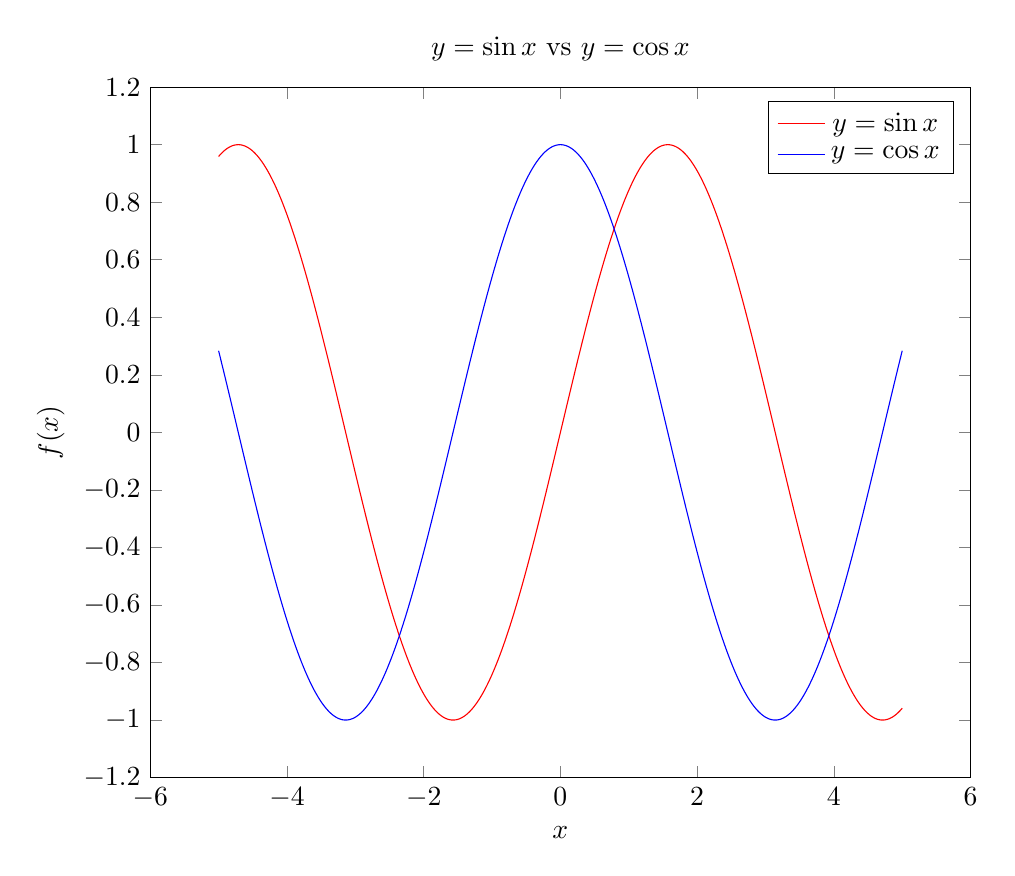
\begin{tikzpicture}
    \begin{axis}[
    title = {$y = \sin x$ vs $y = \cos x$}, xlabel = $x$, ylabel = $f(x)$]
        \addplot[color = red, mark = none, samples = 1000]{sin(deg(x)};
        \addlegendentry{$y = \sin x$}
        \addplot[color = blue, mark = none, samples = 1000]{cos(deg(x))};
        \addlegendentry{$y = \cos x$}
    \end{axis}
\end{tikzpicture}
\subsection{Logarithmic Functions}  
\begin{tikzpicture}
    \begin{axis}[
    title = {$y = \sin x$ vs $y = \cos x$}, xlabel = $x$, ylabel = $f(x)$]
        \addplot[color = red, mark = none, samples = 1000]{log2(x)};
        \addlegendentry{$y = \log_2(x)$}
        \addplot[color = blue, mark = none, samples = 1000]{ln(x)/ln(88)};
        \addlegendentry{$y = \log_{88}(x)$}
    \end{axis}
\end{tikzpicture}
\subsection{Parametric Equations}
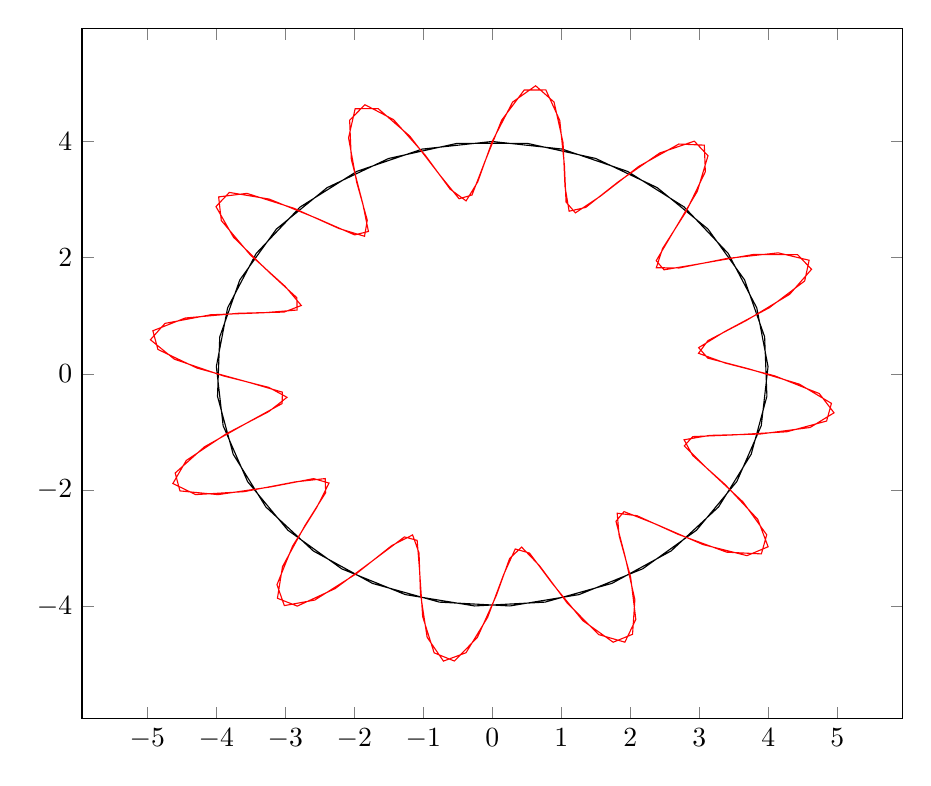
\begin{tikzpicture}
    \begin{axis}
        \addplot [domain=-2*pi:2*pi, samples=50, black] ({4*sin(deg(x))}, {4*cos(deg(x))});
        \addplot [domain=-2*pi:2*pi,samples=200, red]({(4+sin(deg(12*x)))*sin(deg(x))},{(4+sin(deg(12*x)))*cos(deg(x))});
    \end{axis}
\end{tikzpicture}
\subsection{Practice}
\begin{tikzpicture}
    \begin{axis}[
    axis lines=middle,
    ymin=-4.5,ymax=4.5,
    xtick = {-2*pi, -pi, 0, pi, 2*pi},
    xticklabels = {$-2\pi$, $-\pi$, 0, $\pi$, $2\pi$},
    xticklabel style = {anchor = north west}
    ]
        \addplot[domain = -2*pi:2*pi, samples = 500, color = blue, dashed]{tan(deg(x))};
        \addlegendentry{$y = \tan x$}
        \addplot[domain = -2*pi:2*pi, samples = 500, color = red, dashed]{ln(x)};
        \addlegendentry{$y = \ln x$}
    \end{axis}
\end{tikzpicture}
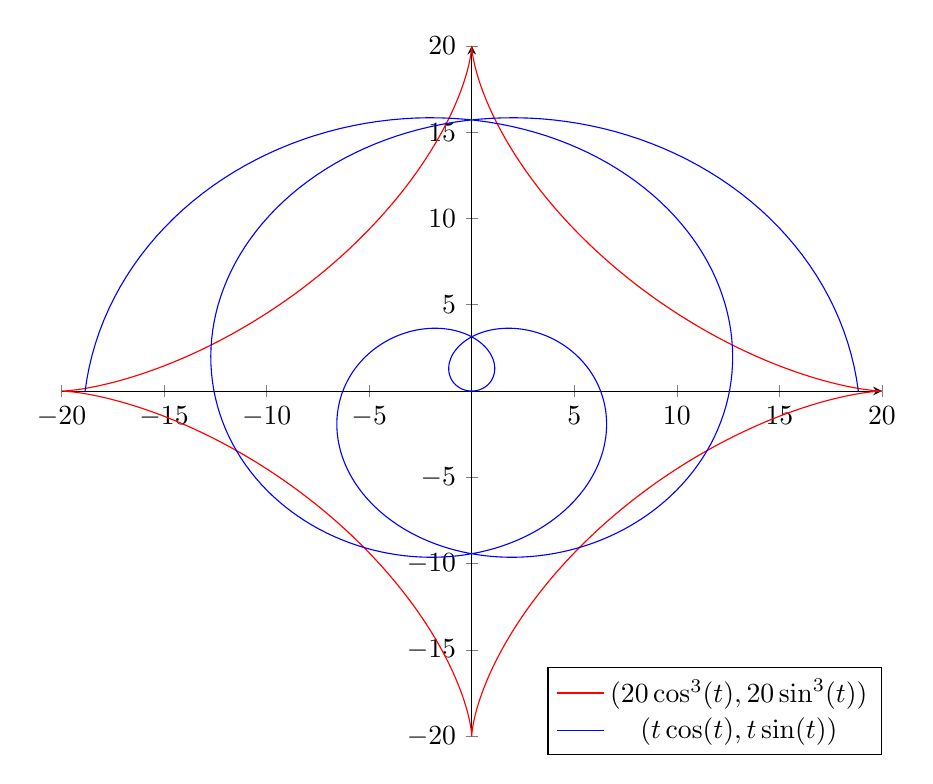
\begin{tikzpicture}
    \begin{axis}[
    axis lines=middle,
    legend style = {
    at = {(1, 0.1)},
    anchor = north east}
    ]
        \addplot[samples = 500, color = red, domain = -3*pi:3*pi]({20*(cos(deg(x)))^3}, {20*(sin(deg(x)))^3});
        \addlegendentry{$(20 \cos^3(t), 20 \sin^3(t))$}
        \addplot[samples = 500, color = blue, domain = -3*pi:3*pi]({2*x*(cos(deg(x)))}, {2*x*(sin(deg(x)))});
        \addlegendentry{$(t \cos (t), t \sin (t))$}
    \end{axis}
\end{tikzpicture}
\section{Creating a 3D-Plot}
\begin{center}
    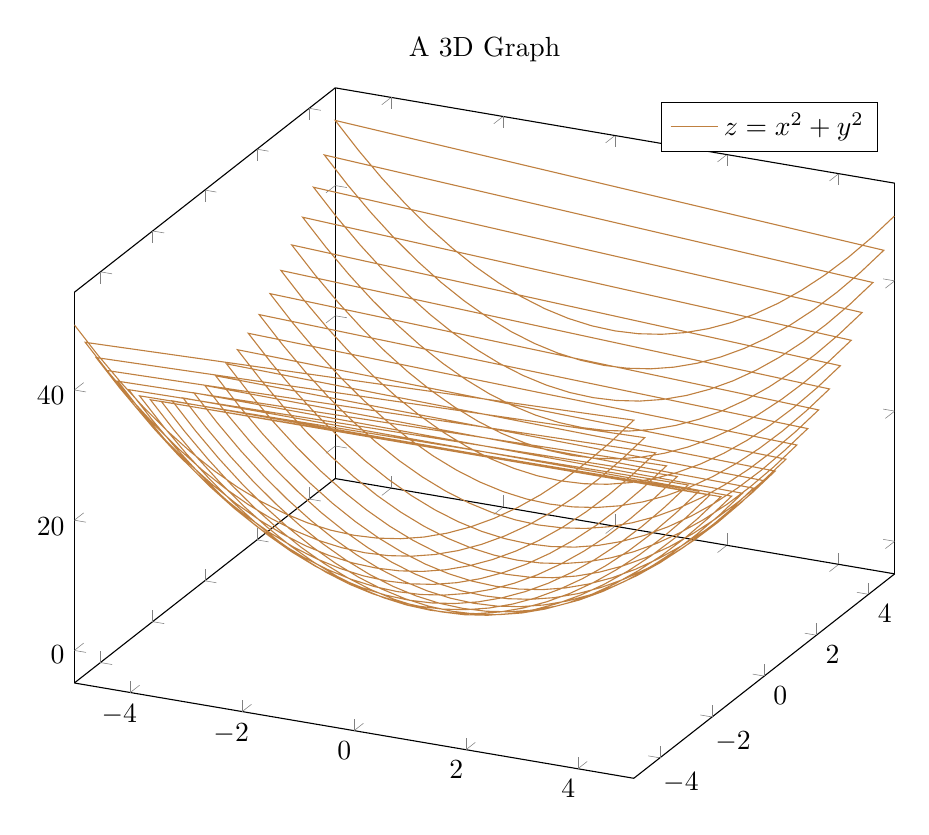
\begin{tikzpicture}
    \begin{axis}[title = {A 3D Graph}]
    \addplot3[color = brown]{x^2+y^2};
    \addlegendentry{$z=x^2+y^2$}
    \end{axis}
    \end{tikzpicture}
\end{center}
\subsection{Types of Surface Plots}
\begin{center}
    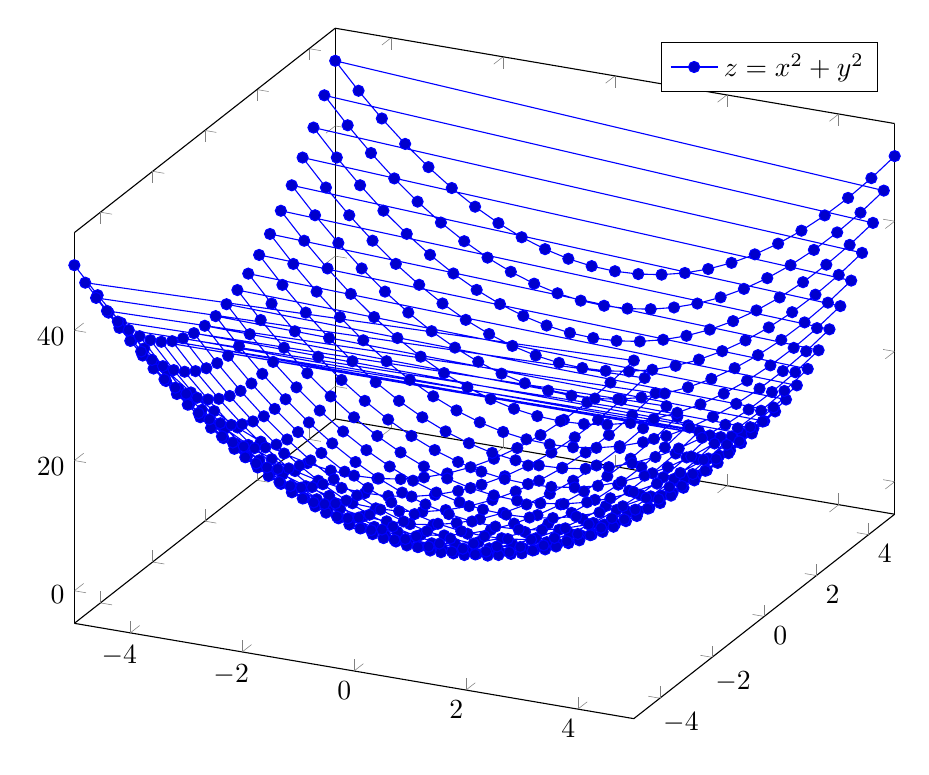
\begin{tikzpicture}
    \begin{axis}
    \addplot3 {x^2+y^2};
    \addlegendentry{$z=x^2+y^2$}
    \end{axis}
    \end{tikzpicture}
\end{center}
\subsubsection{Mesh}
\begin{center}
    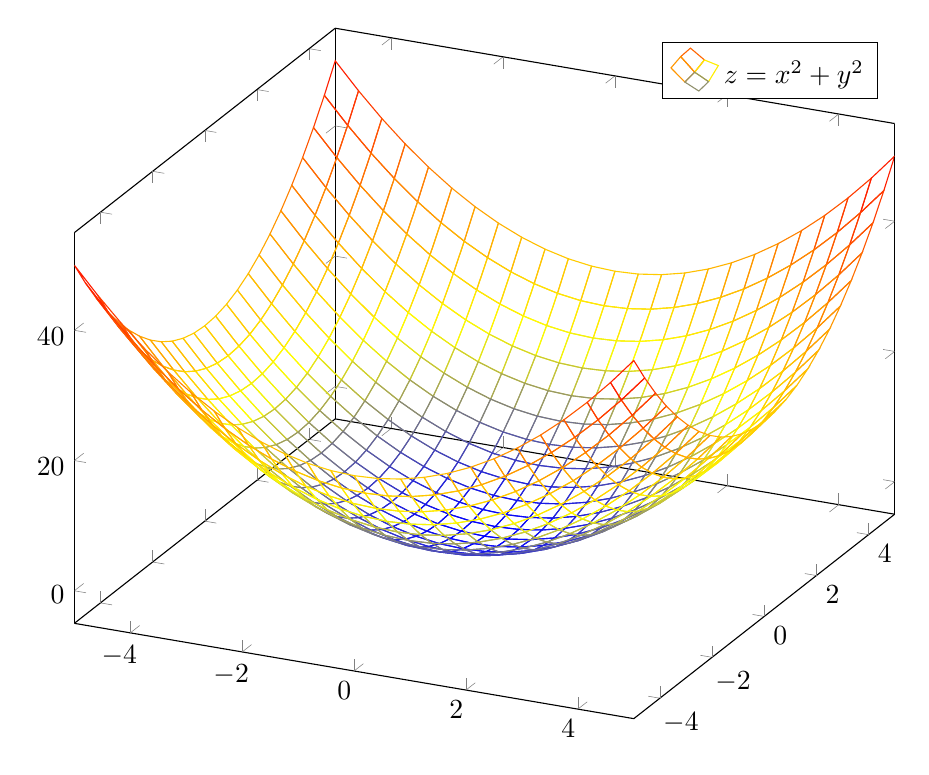
\begin{tikzpicture}
    \begin{axis}
    \addplot3[mesh]{x^2+y^2};
    \addlegendentry{$z=x^2+y^2$}
    \end{axis}
    \end{tikzpicture}
\end{center}
\subsubsection{Surface}
\begin{center}
    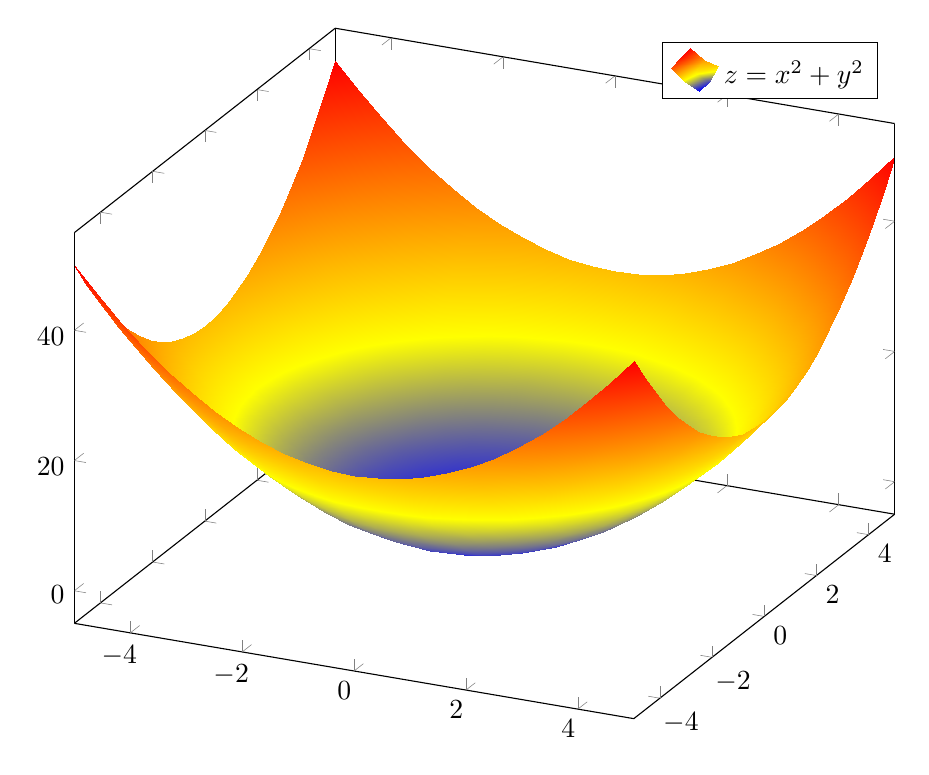
\begin{tikzpicture}
    \begin{axis}
    \addplot3[surf, shader = interp]{x^2+y^2};
    \addlegendentry{$z=x^2+y^2$}
    \end{axis}
    \end{tikzpicture}
\end{center}
\subsection{Inserting a Title}
\begin{center}
    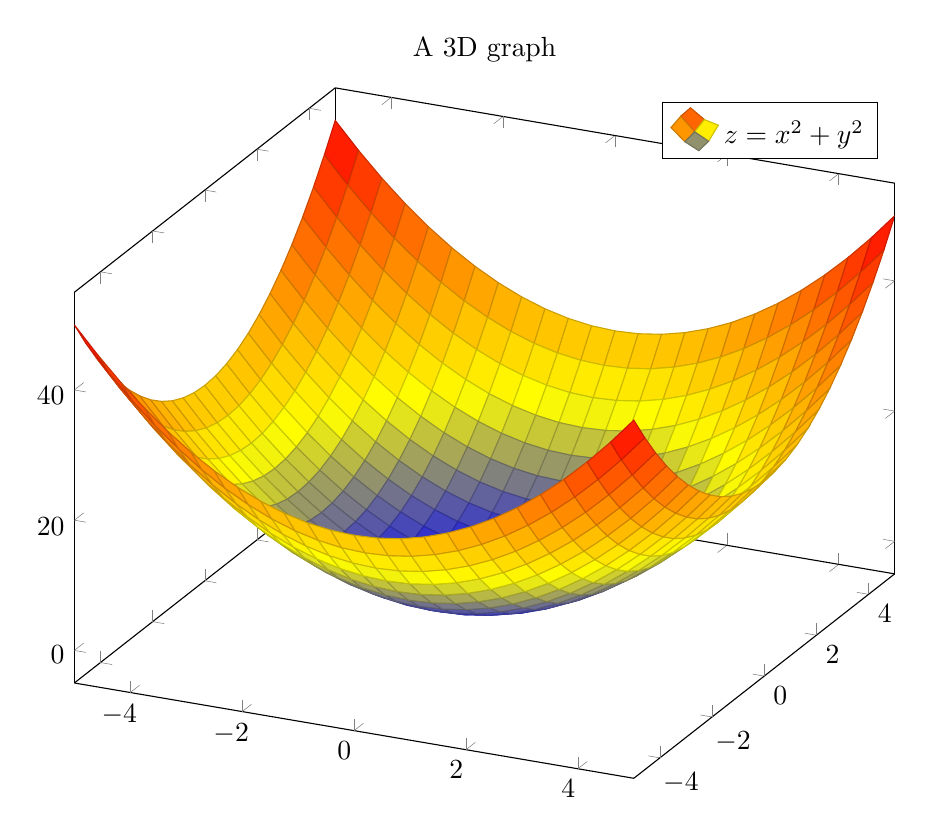
\begin{tikzpicture}
    \begin{axis}[title = {A 3D graph}]
    \addplot3[surf]{x^2+y^2};
    \addlegendentry{$z=x^2+y^2$}
    \end{axis}
    \end{tikzpicture}
\end{center}
\subsection{Changing Perspective}
\begin{center}
    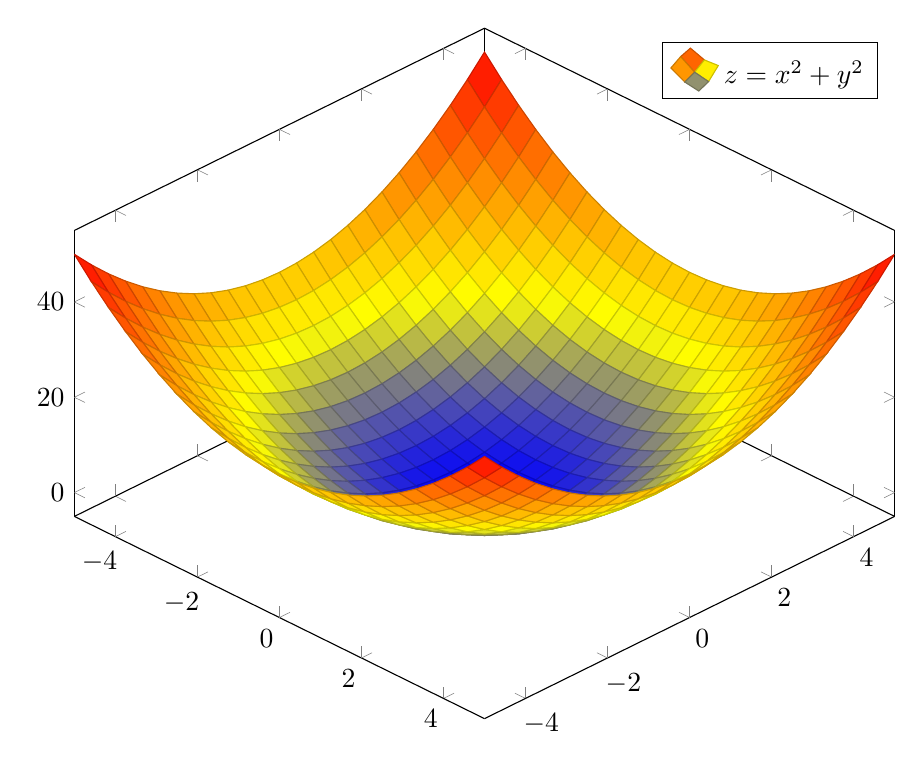
\begin{tikzpicture}
    \begin{axis}[view = {45}{45}]
    \addplot3[surf]{x^2+y^2};
    \addlegendentry{$z=x^2+y^2$}
    \end{axis}
    \end{tikzpicture}
\end{center}
\subsection{Types of Color Map}
\begin{center}
    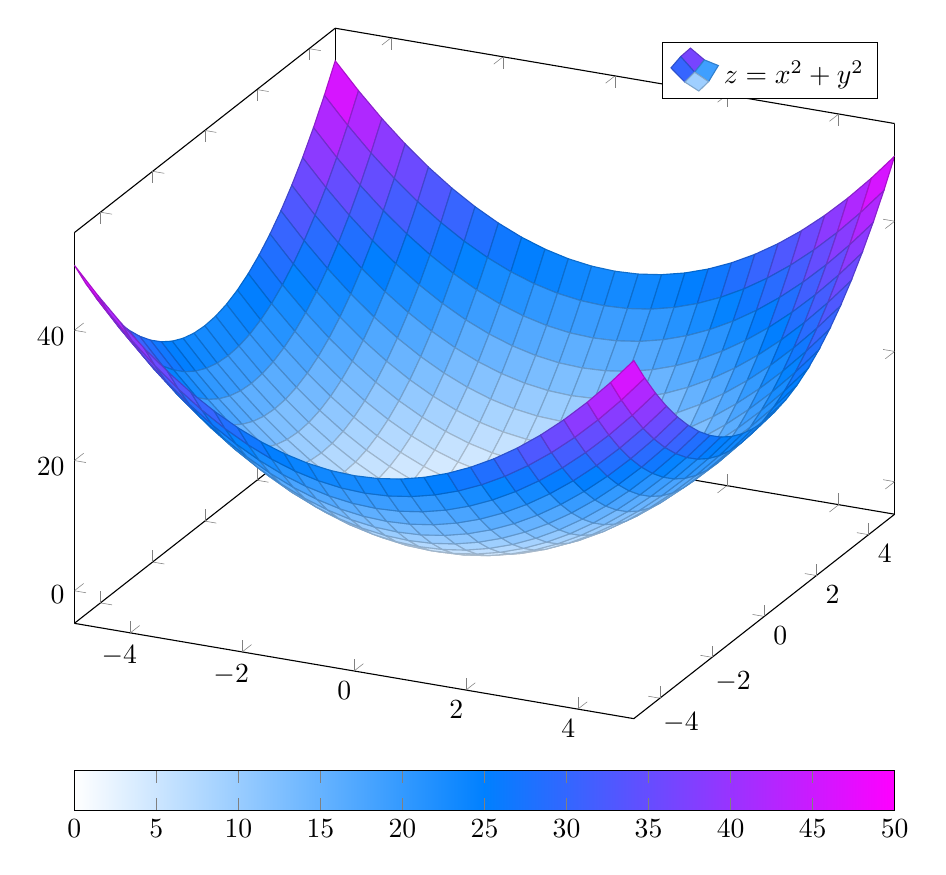
\begin{tikzpicture}
    \begin{axis}[colormap/cool,  colorbar horizontal]
    \addplot3[surf]{x^2+y^2};
    \addlegendentry{$z=x^2+y^2$}
    \end{axis}
    \end{tikzpicture}
\end{center}
\subsection{Solid Colors}
\begin{center}
    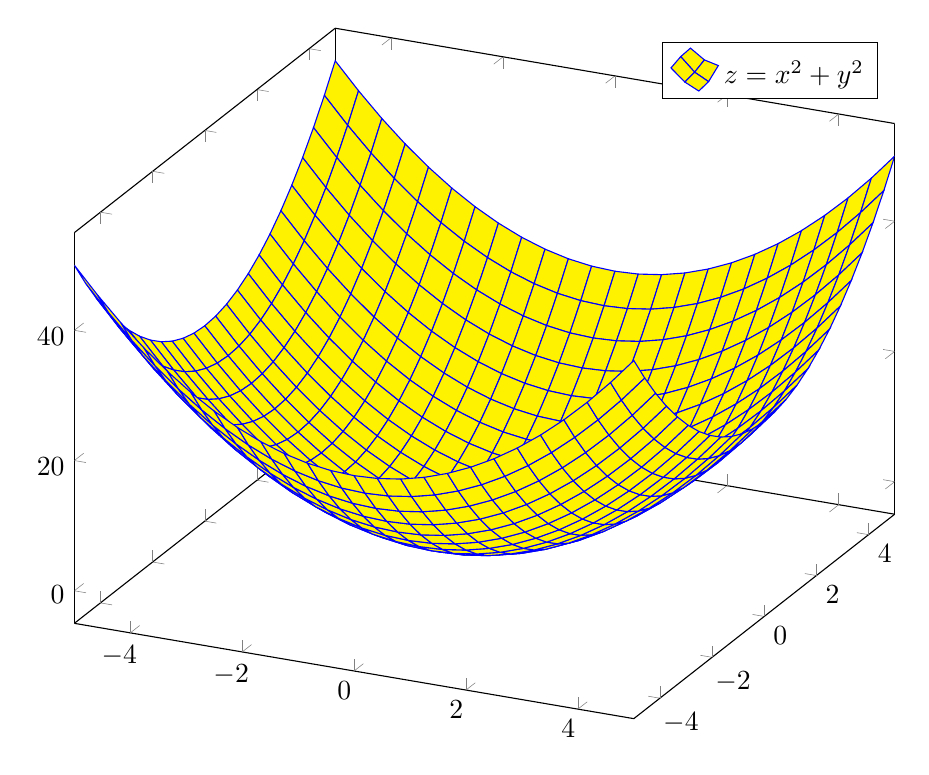
\begin{tikzpicture}
    \begin{axis}
    \addplot3[surf,  color = yellow,
    faceted color = blue]{x^2+y^2};
    \addlegendentry{$z=x^2+y^2$}
    \end{axis}
    \end{tikzpicture}
\end{center}
\subsection{Ranges of Axes}
\begin{center}
    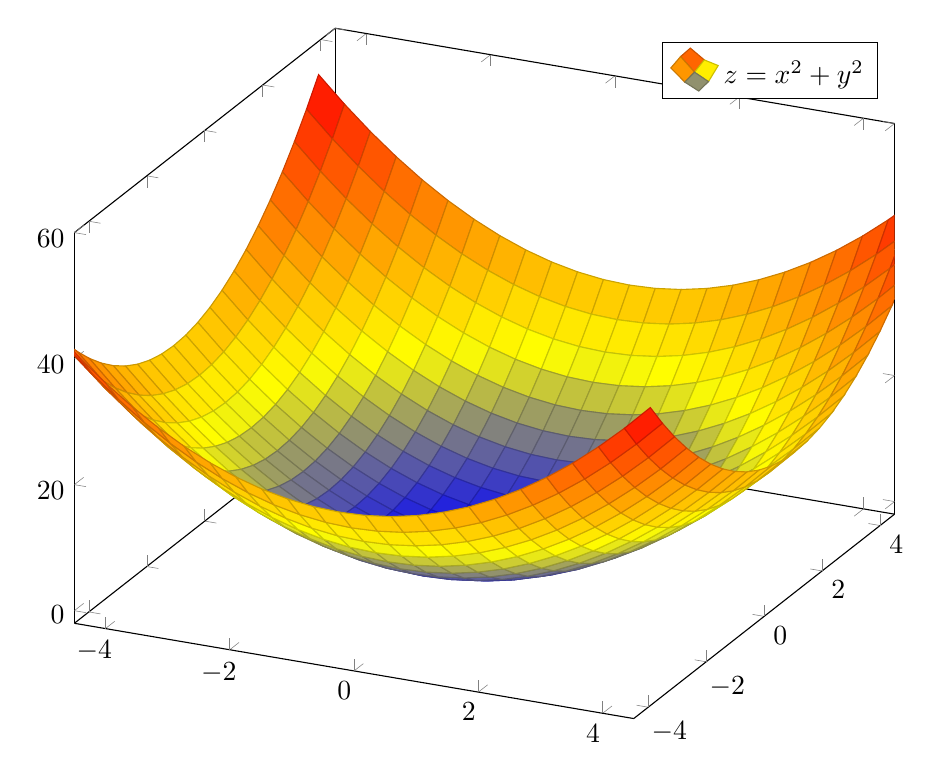
\begin{tikzpicture}
    \begin{axis}[
    xmin = -4.5, xmax = 4.5,
    ymin = -4.5, ymax = 4.5,
    zmin = -2, zmax = 60
    ]
    \addplot3[surf]{x^2+y^2};
    \addlegendentry{$z=x^2+y^2$}
    \end{axis}
    \end{tikzpicture}
\end{center}
\subsection{Axis Position}
\begin{center}
    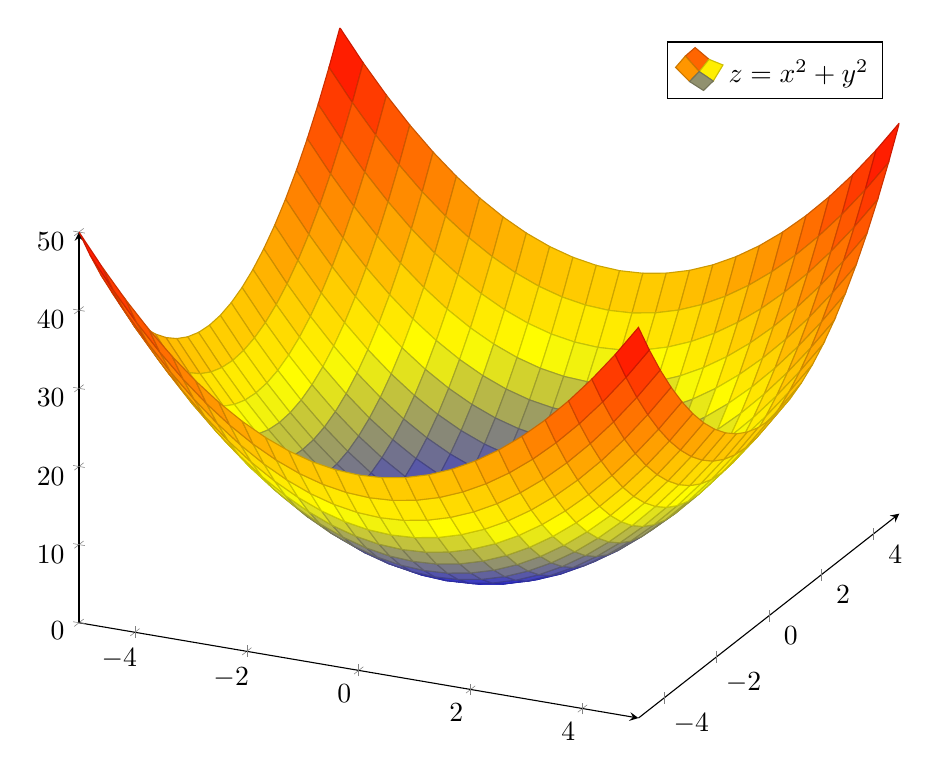
\begin{tikzpicture}
    \begin{axis}[axis lines=left]
    \addplot3[surf]{x^2+y^2};
    \addlegendentry{$z=x^2+y^2$}
    \end{axis}
    \end{tikzpicture}
\end{center}
\subsection{Axes Labels & Ticks}
\begin{center}
    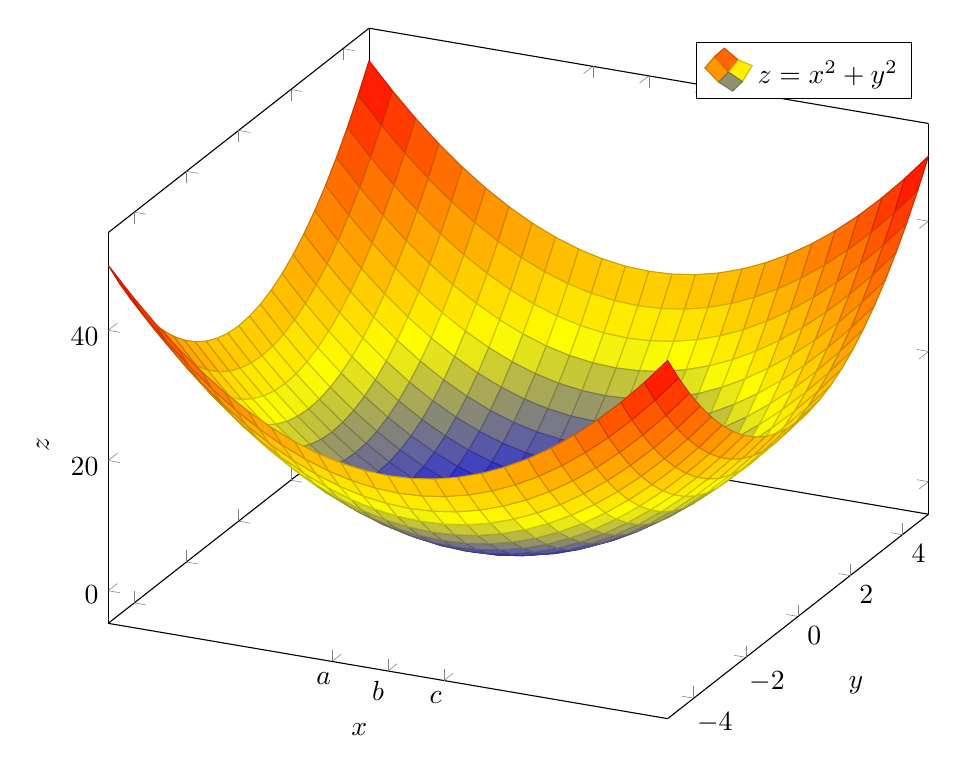
\begin{tikzpicture}
    \begin{axis}[
    xlabel = $x$, ylabel = $y$,  zlabel = $z$, xtick = {-1,0,1},  xticklabels = {$a$, $b$, $c$}
    ]
    \addplot3[surf]{x^2+y^2};
    \addlegendentry{$z=x^2+y^2$}
    \end{axis}
    \end{tikzpicture}
\end{center}
\subsection{Major Gridlines}
\begin{center}
    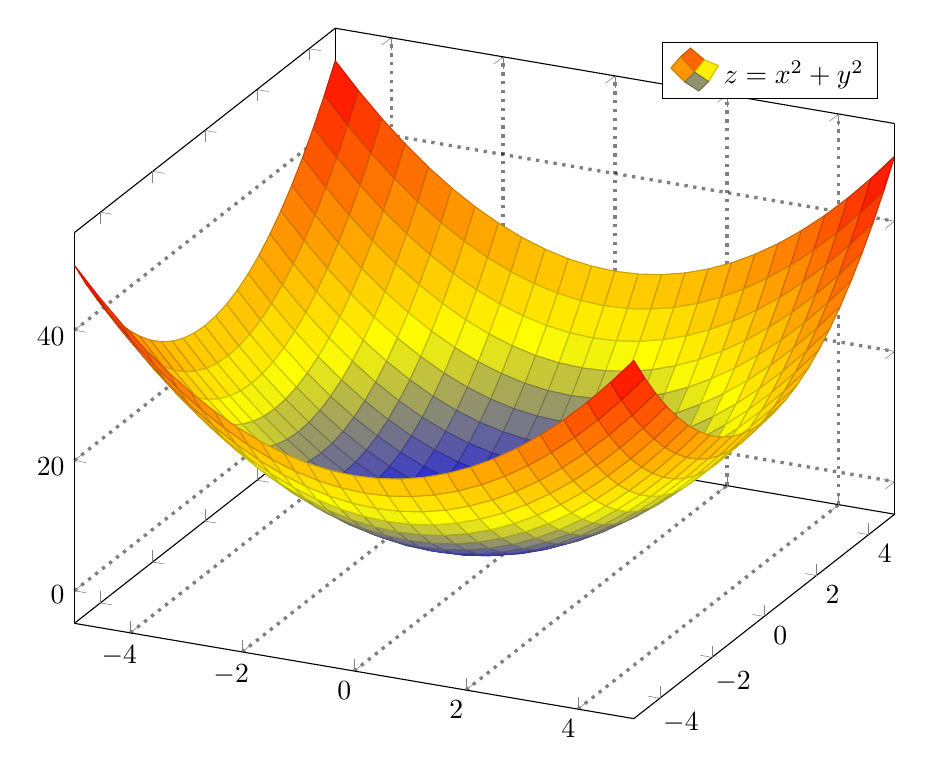
\begin{tikzpicture}
    \begin{axis}[  xmajorgrids = true,  zmajorgrids = true,  grid style = {very thick, dotted, color = black, opacity = 0.5}]
    \addplot3[surf]{x^2+y^2};
    \addlegendentry{$z=x^2+y^2$}
    \end{axis}
    \end{tikzpicture}
\end{center}
Line Style: solid, (loosely or densely) dotted/dashed\\
Thickness: ultra thick/thin, very thick/thin, thick/thin
\subsection{Samples}
\begin{center}
    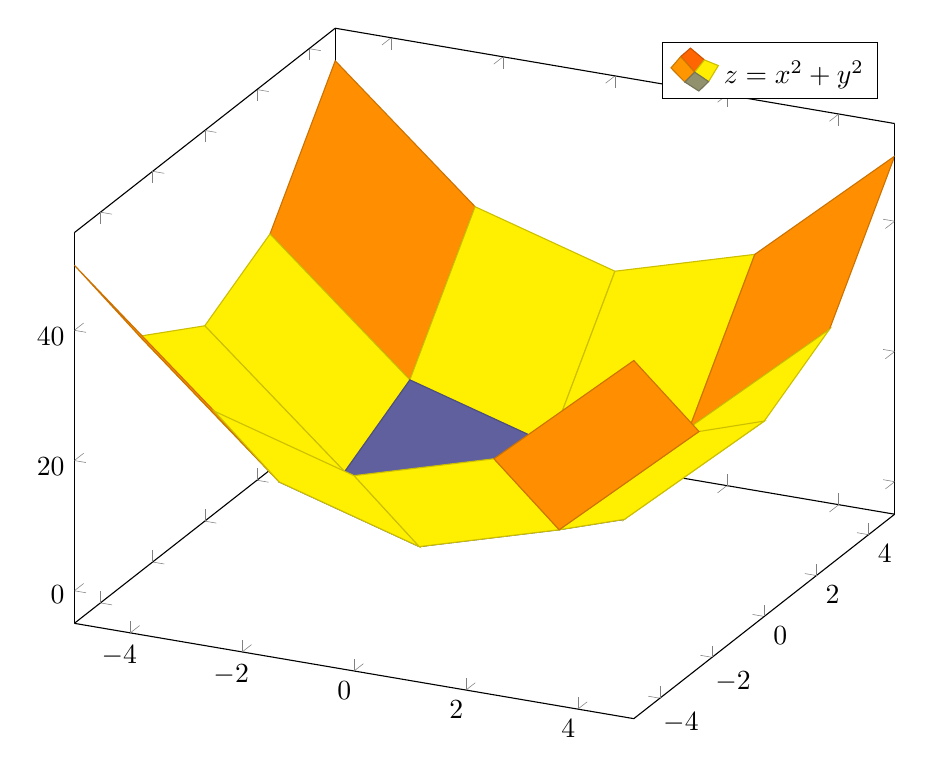
\begin{tikzpicture}
    \begin{axis}
    \addplot3[surf, samples = 5]{x^2+y^2};
    \addlegendentry{$z=x^2+y^2$}
    \end{axis}
    \end{tikzpicture}
\end{center}
\subsection{Domains}
\begin{center}
    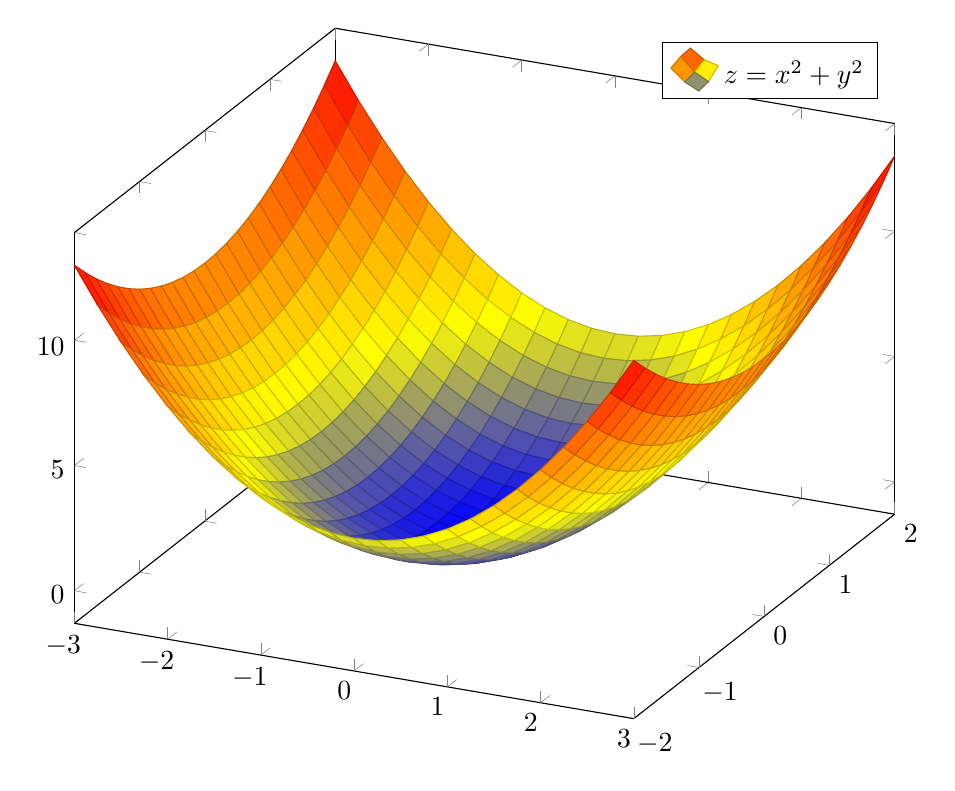
\begin{tikzpicture}
    \begin{axis}
    \addplot3[surf, domain = -3:3, domain y = -2:2]{x^2+y^2};
    \addlegendentry{$z=x^2+y^2$}
    \end{axis}
    \end{tikzpicture}
\end{center}
\subsection{Example: Creating a 3D Parametric Plot}
\begin{center}
    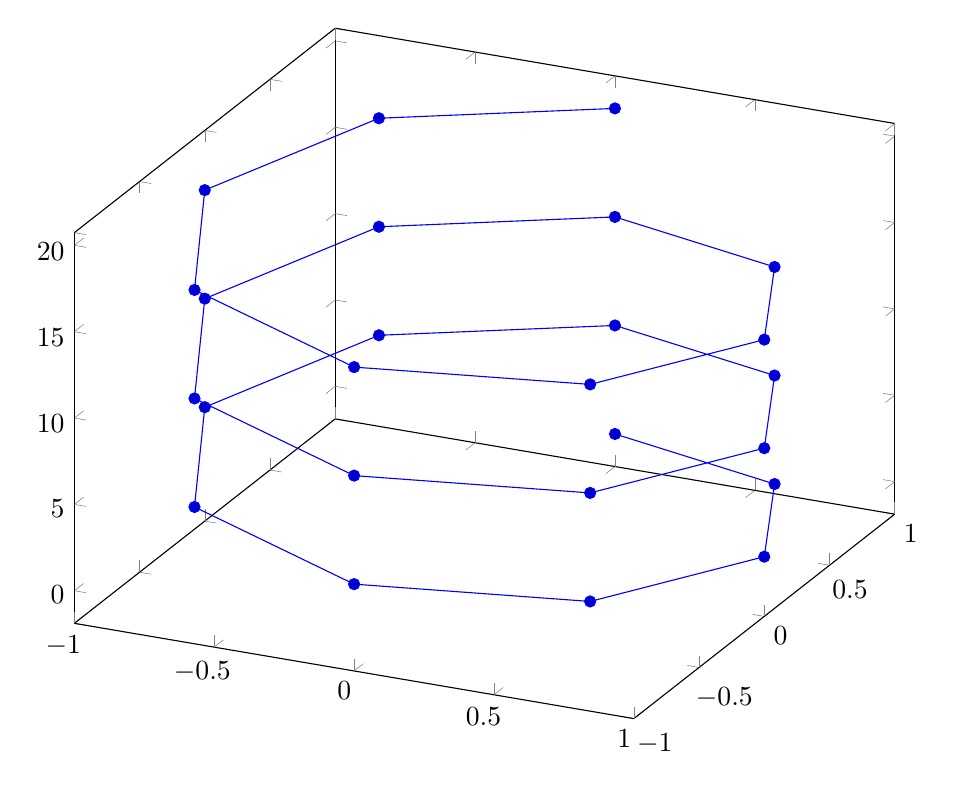
\begin{tikzpicture}
    \begin{axis}
    \addplot3+[domain = 0:6*pi, samples y = 0]
    ({sin(deg(x))}, {cos(deg(x))}, {x});
    \end{axis}
    \end{tikzpicture}
\end{center}
\subsection{Other Customisations for Parametric Plots}
\begin{center}
    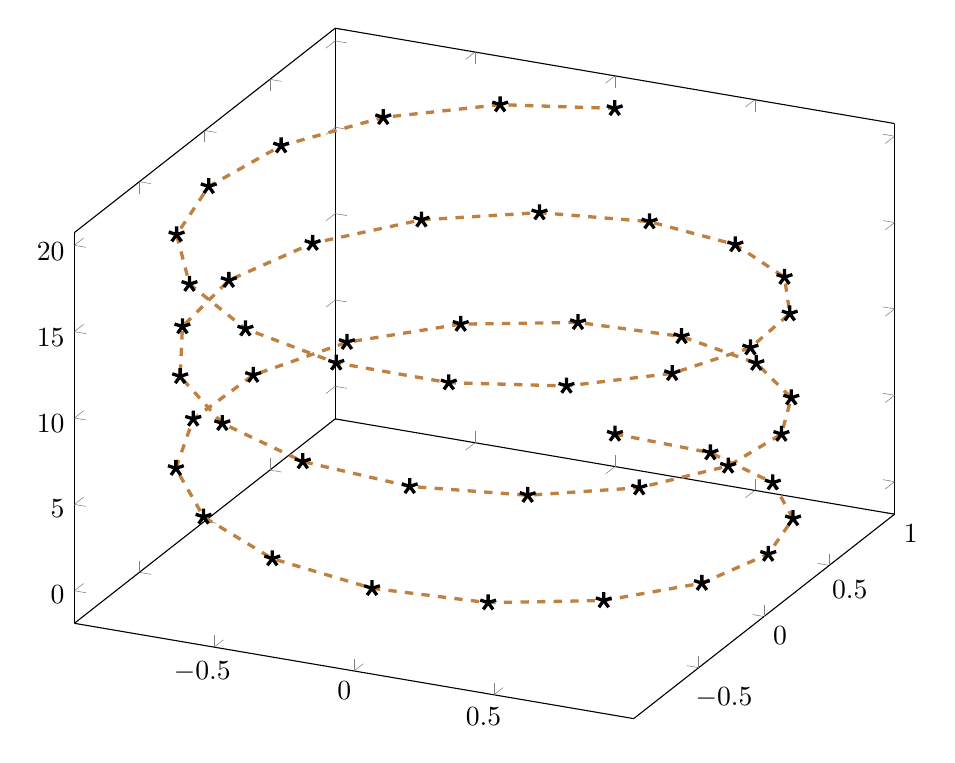
\begin{tikzpicture}
    \begin{axis}
    \addplot3[samples = 50, domain = 0:6*pi, samples y = 0,  style = {very thick, dashed},  color = brown, mark = star, mark options = {black, scale = 2},]  ({sin(deg(x))}, {cos(deg(x))}, {x});
    \end{axis}
    \end{tikzpicture}
\end{center}
\subsection{Practice}
\begin{center}
    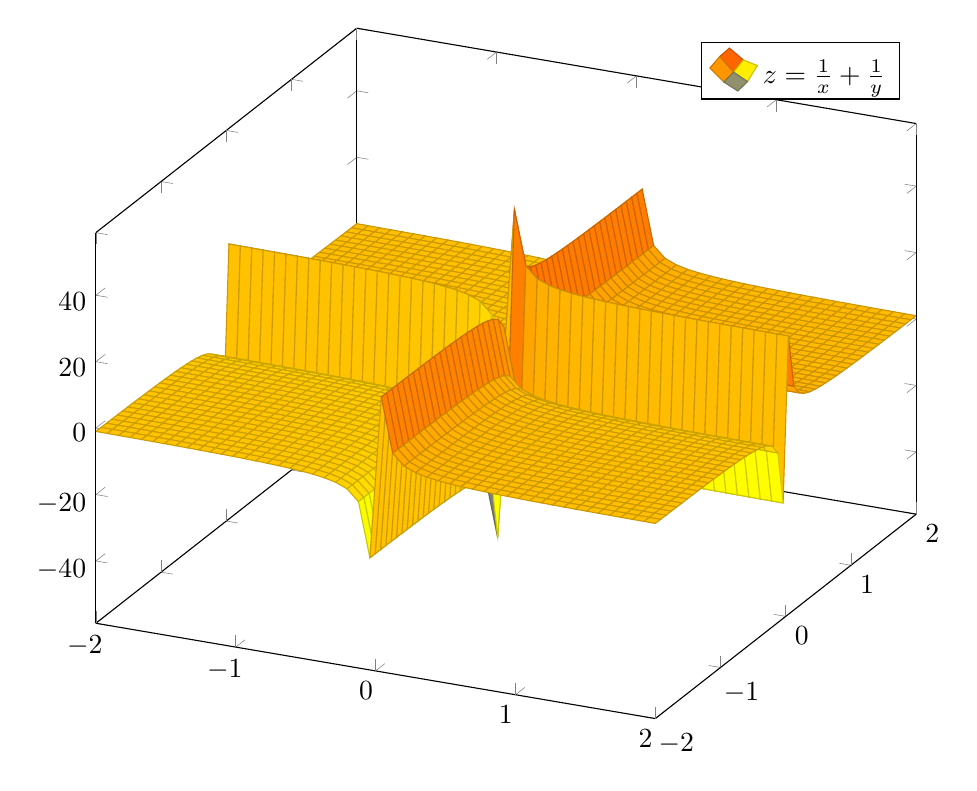
\begin{tikzpicture}
    \begin{axis}
    \addplot3[domain = -2:2, domain y = -2:2, surf,  samples=50]{1/x + 1/y};
    \addlegendentry{$z = \frac{1}{x} + \frac{1}{y}$}
    \end{axis}
    \end{tikzpicture}
\end{center}
\begin{center}
    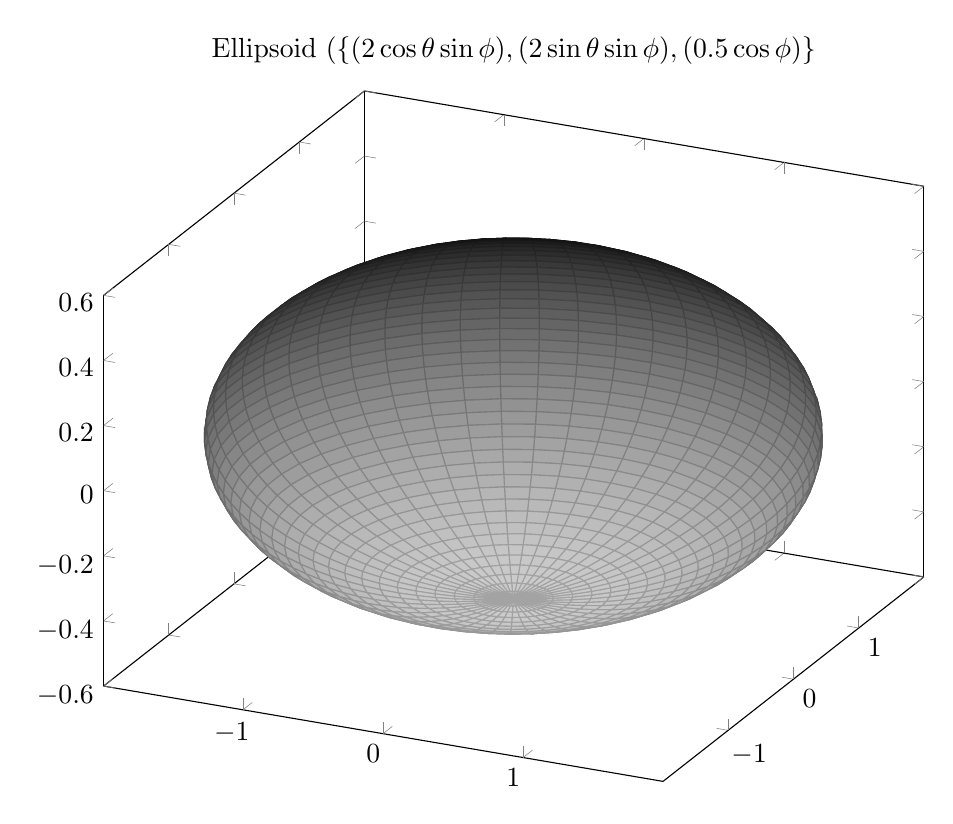
\begin{tikzpicture}
    \begin{axis}[title = {Ellipsoid ($\{(2\cos \theta \sin \phi), (2 \sin \theta \sin \phi), (0.5 \cos \phi)\}$},
    colormap={}{ gray(0cm)=(0.8); gray(1cm)=(0);}]
    \addplot3[surf, samples = 50, domain=0:2*pi,y domain=0:pi]({2*cos(deg(x))*sin(deg(y))}, {2*sin(deg(x))*sin(deg(y))}, {0.5*cos(deg(y))});
    \end{axis}
    \end{tikzpicture}
\end{center}
\section{Bar Plots}
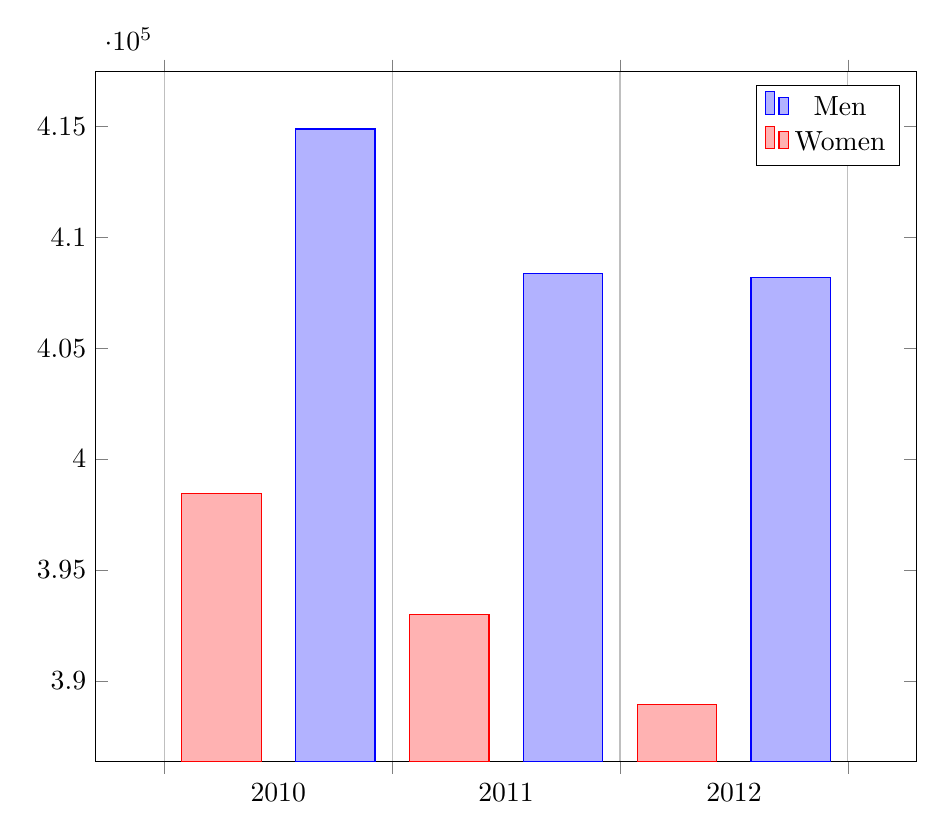
\begin{tikzpicture}
    \begin{axis}[
        ybar interval=0.7,
        x tick label style={/pgf/number format/1000 sep=}]
    \addplot 
    	coordinates {(2012,408184) (2011,408348)
    		 (2010,414870) (2009,412156)};
    \addplot 
    	coordinates {(2012,388950) (2011,393007) 
    		(2010,398449) (2009,395972)};
    \legend{Men,Women}
    \end{axis}
\end{tikzpicture}
\end{document}